\documentclass[12pt,a4paper]{cibb}

\usepackage{subfigure,graphicx}
\usepackage{amsmath,amsfonts,latexsym,amssymb,euscript,xr}
\usepackage{enumitem}


% Package to generate and customize Algorithm as per ACM style
\usepackage[ruled, linesnumbered, noend]{algorithm2e}
\renewcommand{\algorithmcfname}{Listing}
\SetAlFnt{\small}
\SetAlCapFnt{\small}
\SetAlCapNameFnt{\small}
\SetAlCapHSkip{0pt}
\IncMargin{-\parindent}


\title{\large $\ $\\ \bf MODIFICATION OF VALIANT'S PARSING ALGORITHM FOR STRING-SEARCHING PROBLEM}

\author{Yuliya Susanina$^{(1),(2)}$, Anna Yaveyn$^{(1)}$, Semyon Grigorev$^{(1),(2)}$}
\address{$\ $\\(1) Saint Petersburg State University, 7/9 Universitetskaya nab., St. Petersburg, 199034 Russia\\
jsusanina@gmail.com,
anya.yaveyn@yandex.ru
\\
%
\bigskip
(2) JetBrains Research, Universitetskaya emb., 7-9-11/5A, St.Petersburg, Russia\\
semen.grigorev@jetbrains.com
}


\abstract{Context-free grammar, string-matching, Valiant's algorithm, secondary structure, parsing.
\\[17pt]
{\bf Abstract.} 
Some string-matching problems can be reduced to parsing: verification whether some subsequence can be derived in the given grammar. 
To apply parser-based solutions to such area as bioinformatics, one needs to improve parsing techniques so that the processing of a large amount of data was possible.
The most asymptotically efficient parsing algorithm that can be applied to any context-free grammar is a matrix-based algorithm proposed by Valiant.
This paper presents a modification of the Valiant’s algorithm, which allows one to simplify highly parallel implementation, and efficiently utilize modern massively-parallel hardware. 
Moreover, the modified version decreases a large amount of excessive computations and accelerates the substrings searching. }

\begin{document}
\thispagestyle{myheadings}
\pagestyle{myheadings}
\markright{\tt Proceedings of CIBB 2019}%check year

\chapter*{Введение}                         % Заголовок
\addcontentsline{toc}{chapter}{Введение}    % Добавляем его в оглавление
\textbf{Актуальность работы}

Статический анализ исходного кода является известной техникой  получения знаний о программе без её исполнения ~\cite{StaticCodeAnalysis3,StaticCodeAnalysis2,StaticCodeAnalysis1}. Статический анализ является неотъемлемой частью многих процессов, связанных с разработкой программного обеспечения (ПО), и может использоваться, например, для упрощения работы с кодом с помощью подсветки синтаксиса языка в программах, навигации по коду, реализации контекстных подсказок. Более того, статический анализ используется для обнаружения ошибок на ранних стадиях разработки, до запуска программы, а также для поиска различных семантических ошибок, которые не могут быть определены обычным синтаксическим анализом.  Также, статический анализ используется при решении задач трансформации исходного кода и реинжиниринге~\cite{reengANT}. Однако во многих языках программирования имеются конструкции, которые существенно затрудняют статический анализ. 

Например, широко используются динамические встроенные языки --- приложение, созданное на одном языке, генерирует программу на другом языке и передаёт её на выполнение в соответствующее окружение. Примерами могут служить динамические SQL-запросы к базам данных из приложений на Java, С++, С\#, формирование HTML-страниц в PHP-приложениях~\cite{DSQLISO,JSP,PHPmySQL}. Генерируемый код собирается из строк таким образом, чтобы в момент выполнения результирующая строка представляла собой корректную программу. Примеры использования встроенных языков представлены в листингах~\ref{lst:dsql1},~\ref{lst:JsJava} и~\ref{lst:PhPSqlHtml}. Следует отметить, что одна программа может генерировать код на нескольких языках (см. листинг~\ref{lst:PhPSqlHtml}). При этом возможно получение частей кода из разных источников (например, учитывать текстовый ввод пользователя, что часто используется для задания фильтров при конструировании SQL-запросов). Использование динамически формируемых программ  позволяет избежать дополнительных накладных расходов, присущих таким технологиям, как ORM\footnote{ORM или Object-Relational Mapping --- технология программирования, которая связывает базы данных с концепциями объектно-ориентированных языков программирования~\cite{ORM}.}, и достичь высокой производительности. Благодаря этому использование динамически генерируемых программ получило широкое распространение и применяется до сих пор. Вместе с этим, несмотря на появление новых технологий, динамическая генерация SQL-запросов активно используется и в настоящее время~\cite{DSQLInActiveUse}.

\fvset{frame=lines,framesep=5pt,fontsize=\small}\

\begin{listing}
    \begin{pyglist}[language=sql,numbers=left,numbersep=5pt]

CREATE PROCEDURE [dbo].[MyProc]  @TABLERes   VarChar(30)
AS
    EXECUTE ('INSERT INTO ' + @TABLERes + ' (sText1)' +
             ' SELECT ''Additional condition: '' + sName' +
             ' from #tt where sAction = ''1000000''')
GO
    \end{pyglist}
\caption{Код с использованием динамического SQL}
\label{lst:dsql1}
\end{listing} 
 
\fvset{frame=lines,framesep=5pt}
\begin{listing}
    \begin{pyglist}[language=java,numbers=left,numbersep=5pt]
import javax.script.*;  
public class InvokeScriptFunction {  
    public static void main(String[] args) throws Exception {  
        ScriptEngineManager manager = new ScriptEngineManager();  
        ScriptEngine engine = manager.getEngineByName("JavaScript");  
        // JavaScript code in a String  
        String script = 
            "function hello(name) { print('Hello, ' + name); }";  
        // evaluate script  
        engine.eval(script);  
        // javax.script.Invocable is an optional interface.  
        // Check whether your script engine implements or not!  
        // Note that the JavaScript engine implements
        // Invocable interface.  
        Invocable inv = (Invocable) engine;  
        // invoke the global function named "hello"  
        inv.invokeFunction("hello", "Scripting!!" );  
    }  
}
    \end{pyglist}
\caption{Вызов JavaScript из Java}
\label{lst:JsJava}
\end{listing}


\fvset{frame=lines,framesep=5pt}
\begin{listing}
    \begin{pyglist}[language=php,numbers=left,numbersep=5pt]

<?php
    // Embedded SQL
    $query = 'SELECT * FROM ' . $my_table; 
    $result = mysql_query($query);
    
    // HTML markup generation
    echo "<table>\n";
    while ($line = mysql_fetch_array($result, MYSQL_ASSOC)) {
        echo "\t<tr>\n";    
        foreach ($line as $col_value) {
            echo "\t\t<td>$col_value</td>\n";
        }
        echo "\t</tr>\n";
    }
    echo "</table>\n";
?>
    \end{pyglist}
\caption{Использование нескольких встроенных в PHP языков (MySQL, HTML)}
\label{lst:PhPSqlHtml}
\end{listing}



Динамически формируемые выражения часто конструируются с помощью таких операций, как конкатенация в циклах или условных предложениях, или в рекурсивных процедурах. Это затрудняет статический анализ и приводит к получению множества возможных значений для каждого выражения в момент выполнения. Вследствие этого фрагменты динамически формируемого кода воспринимаются компилятором исходного языка как простые строки, не подлежащие дополнительному анализу, а это, в свою очередь, приводит к высокой вероятности возникновения ошибок во время выполнения программы. В худшем случае такая ошибка не приведёт к прекращению работы приложения, что указало бы на проблемы, однако целостность данных при этом может оказаться нарушена. Более того, использование динамически формируемых выражений затрудняет не только разработку информационных систем, так и также и реинжиниринг, поскольку в последнем случае важно автоматизировать перенос системы на новые зыки и платформы, что невозможно без качественного статического анализа. Например, при наличии в коде приложения динамически формируемых SQL-запросов нельзя точно ответить на вопрос о том, с какими элементами базы данных не взаимодействует система, и удалить их. При переносе такой системы на другую СУБД необходимо гарантировать, что для всех динамически формируемых выражений значение в момент выполнения будет корректным кодом на языке новой СУБД~\cite{JSquash}. Следует отметить, что отсутствие статического анализа динамически формируемых программ не позволяет реализовывать для них стандартную функциональность интегрированных сред разработки (Integrated Development Environment, IDE) --- подсветку синтаксиса и автодополнение, рефакторинг кода и т.д. Такая функциональность значительно упрощает процесс разработки и отладки приложений и полезна не только для основного языка, но и для встроенных языков. 

Для решения всех перечисленных выше задач необходимы инструменты, проводящие статический анализ динамически формируемых программ. Такой анализ может дать существенную информацию о таких программах, поскольку редко встречается ситуация полной динамической неопределённости (например, при создании динамических программ исключительно на основе пользовательского ввода). В большинстве случаев, имея программу, генерирующую динамические вставки, с помощью статического анализа можно получить достаточно информации для решения поставленных выше задач. Решению этой проблемы и посвящена данная диссертационная работа. 


\textbf{Степень разработанности темы}

Существуют классические исследования, посвященные разработке компиляторов --- работы А.~Ахо~\cite{Dragon}, А.~Брукера~\cite{CompilerCompiler}, С.~Джонсона~\cite{yaccBook},  Б.К.Мартыненко~\cite{Martinenko1, Martinenko2}  и др.  Однако содержащиеся там алгоритмы синтаксического анализа не могут быть применены к решению задачи анализа динамически формируемых программ, поскольку предназначены для обработки входных данных, представимых в видн линейной последовательности символов, а такое представление динамически формируемых программ не всегда возможно.

Методы обобщённого синтаксического анализа, лежащие в основе данной работы, изложены в трудах таких учёных как Масару Томита (Masaru Tomita)~\cite{Tomita}, Элизабет Скотт (Elizabeth Scott) и Адриан Джонстон (Adrian Johnstone)~\cite{RNGLR,RIGLR} из университета Royal Holloway (Великобритания), Ян Рекерс (Jan Rekers, University of Amsterdam)~\cite{SPPF}, Элко Виссер (Eelco Visser)~\cite{RNGLRSyntaxerror2,RNGLRSyntaxerror3} и других.

Анализу динамически формируемых строковых выражений посвящены работы таких зарубежных учёных как Кюнг-Гу Дох (Kyung-Goo Doh)~\cite{LrAbstract1,LrAbstract2,LRAbstractParsingSema}, Ясухико Минамиде (Minamide Yasuhiko)~\cite{PHPSA}, Андерс Мёллер (Anders M{\o}ller)~\cite{JSA} и отечественных учёных А.А.~Бреслава~\cite{Alvor1,Alvor2} и других. Хорошо изучены вопросы проверки корректности динамически формируемых выражений и поиска фрагментов кода, уязвимых для SQL-инъекций~\cite{SQLInjection,Dasgupta:2009:SAF:1546683.1547548}. Однако данные работы исследуют отдельные аспекты проблемы статического анализа динамически формируемых программ, оставляя в стороне создание готовых алгоритмов (в частности, не строят структурное представление анализируемых программ). В связи с этим возникают проблемы масштабируемости данных результатов, например, создание на их основе более сложных видов статического анализа.

Так же важным является предоставление компонентов, упрощающих создание новых инструментов для решения конкретных задач. Данных подход хорошо исследован в области разработки компиляторов, где широкое распространение получили генераторы анализаторов и пакеты стандартных библиотек (работы А.~Ахо~\cite{Dragon}, А.~Брукера~\cite{CompilerCompiler}, С.~Джонсона~\cite{yaccBook} и др.). 

В работах отечественных учёных М.Д.~Шапот и Э.В.~Попова~\cite{DynamicDSQLTranslation}, а так же зарубежных учёных Антони Клеви (Anthony Cleve), Жан-Люк Эно (Jean-Luc Hainaut)~\cite{DSQLReverseEngineering}, Йост Виссер (Joost Visser)~\cite{DSQLQualityMesure} и других рассматриваются различные аспекты реинжиниринга информационных систем, использующих встроенные SQL-запросы, однако не формулируется общего метода для решения таких задач. Этот вопрос также не затрагивается в классических работах, посвященных реинжиниригу~\cite{SoftwareReeng1, reengANT, SoftwareReeng2, SoftwareReeng3}. Однако разработка такого метода является актуальной задачей.

Таким образом, актуальной является задача дальнейшего исследования статического анализа динамически формируемых строковых выражений. Кроме этого важным является решение вопросов практического применения средств анализа динамически формируемого кода: упрощение разработки инструментов анализа и создание методов их применения в реинжиниринге программного обеспечения.
\textbf{Объект исследования}

Объектом исследования являются методы, алгоритмы и программные средства обработки динамически формируемых программ, а также задача реинжиниринга информационных систем.

\textbf{Цель и задачи диссертационной работы}

\textbf{Целью} данной работы является создание комплексного подхода к статическому синтаксическому анализу динамически формируемых программ.

Достижение поставленной цели обеспечивается решением следующих \textbf{задач}.
\begin{enumerate}
    \item Разработать универсальный алгоритм синтаксического анализа динамически формируемых программ, не зависящий от целевого языка программирования и допускающий реализацию различных видов статического анализа. 
    \item Создать архитектуру инструментария для автоматизации разработки программных средств статического анализа динамически формируемых программ.
    \item Создать метод реинжиниринга динамически формируемых программ.
\end{enumerate}

\textbf{Методология и методы исследования}

Методология исследования основана на подходе к спецификации и анализу формальных языков, активно развивающемуся с 50-х годов 20-го века (см., например, работы Н. Хомского~\cite{chomskyMethod ,chomskySyntactic}). В последствии этот подход получил широкое распространение в областях, связанных с обработкой языков программирования.
Основными элементами данного подхода являются алфавит и грамматика языка, разбиение автоматической обработки языка на выполнение таких шагов как лексический, синтаксический и семантический анализ. Решаемые в связи с этим задачи связаны с поиском эффективных алгоритмов, выполняющих эти шаги. 

В работе применяется алгоритм обобщённого восходящего синтаксического анализа RNGLR~\cite{RNGLR}, созданный Элизабет Скотт (Elizabeth Scott) и Адриан Джонстон (Adrian Johnstone) из университета Royal Holloway (Великобритания). Для компактного хранения леса вывода использовалась структура данных Shared Packed Parse Forest (SPPF), которую предложил Ян Рекерс (Jan Rekers, University of Amsterdam)~\cite{SPPF}.

Доказательство завершаемости и корректности предложенного алгоритма проводилось с применением теории формальных языков, теории графов и теории сложности алгоритмов. Приближение множества значений динамически формируемого выражения строилось в виде регулярного множества, описываемого с помощью конечного автомата.


\textbf{Положения, выносимые на защиту}
\begin{enumerate}
    \item Разработан алгоритм синтаксического анализа динамически формируемых программ, позволяющий обрабатывать произвольную регулярную аппроксимацию множества значений выражения в точке выполнения, реализующий эффективное управление стеком и гарантирующий конечность представления леса вывода. Доказана завершаемость и корректность предложенного алгоритма при обработке регулярной аппроксимации, представимой в виде произвольного конечного автомата без $\varepsilon$-переходов. 
    \item Создана архитектура инструментария для разработки программных средств статического анализа динамически формируемых программ.
    \item Разработан метод анализа и обработки динамически формируемых программ в проектах по реинжинирингу информационных систем. 
\end{enumerate}

\textbf{Научная новизна работы}

Научная новизна полученных в ходе исследования результатов заключается в следующем.

\begin{enumerate}

\item Алгоритм, предложенный в диссертации, отличается от аналогов (работы Андрея Бреслава~\cite{Alvor1, Alvor2}, Кюнг-Гу Дох~\cite{LrAbstract1, LrAbstract2}, Ясухико Минамиде~\cite{PHPSA}) возможностью построения компактной структуры данных, содержащей деревья вывода для всех корректных значений выражения. Это позволяет использовать результаты работы алгоритма для проведения более сложных видов анализа. Алгоритмы, представленные в (JSA~\cite{JSA}~\cite{Alvor1, Alvor2}, PHPSA~\cite{PHPSA}) предназначены только для проверки корректности выражений, основанной на решении задачи о включении одного языка в другой. Выполнение более сложных видов анализа, трансформаций или построения леса разбора не предполагается. 

\item Новизна представленной архитектуры заключается в том, что она позволяет создать платформу для разработки целевых инструментов, решающих широкий круг задач анализа динамически формируемого кода. Существующие архитектуры готовых инструментов (JSA, PHPSA, Alvor, Varis) предназначены для решения конкретных задач для определённых языков. Решение новых задач или поддержка других языков с помощью этих инструментов затруднены ввиду ограничений, накладываемых архитектурой и возможностями используемого алгоритма анализа. 

\item Метод анализа и обработки встроенного программного кода в проектах по реинжинирингу информационных систем предложен впервые. К.В.~Ахтырченко и Т.П.~Сорокваша отмечают~\cite{SoftwareReengMethods}, что существующие работы в области реинжиниринга программного обеспечения либо содержат высокоуровневые решения, не касающиеся деталей, важных при решении прикладных задач (например, работы К. Вагнера~\cite{SoftwareReeng3}, Х. Миллера~\cite{SoftwareReeng2}), либо являются набором подходов к решению конкретных задач (например, работы~\cite{SoftwareReeng1, reengANT, boulychev}). При этом, встроенный программный код часто не учитывается. С другой стороны, работы М.Д.~Шапот и Э.В.~Попова~\cite{DynamicDSQLTranslation}, С.Л.~Трошина~\cite{reengANT}, А.~Клеви~\cite{DSQLReverseEngineering}  посвящены решению конкретных задач обработки встроенного программного кода в контексте реинжиниринга информационных систем, но не предлагают обобщённого и масштабируемого метода.

\end{enumerate}


\textbf{Теоретическая и практическая значимость работы}

Теоретическая значимость диссертационного исследования заключается в разработке формального алгоритма синтаксического анализа динамически формируемого кода, решающего задачу построения конечного представления леса вывода, не решенную полностью ранее, а также в формальном доказательстве завершаемости и корректности разработанного алгоритма. 

На основе полученных в работе научных результатов был разработан инструментарий (Software Development Kit, SDK), предназначенный для создания средств статического анализа динамически формируемых программ. 
С использованием разработанного инструментария было реализовано расширение к инструменту ReSharper (ООО ``ИнтеллиДжей Лабс'', Россия), предоставляющее поддержку встроенного T-SQL в проектах на языке программирования C\# в среде разработки Microsoft Visual Studio. Так же было выполнено внедрение результатов работы в промышленный проект по переносу хранимого SQL-кода с MS-SQL Server 2005 на Oraclе 11gR2 (ЗАО ``Ланит-Терком'', Россия). 

\textbf{Степень достоверности и апробация результатов}

Достоверность и обоснованность результатов исследования опирается на использование формальных методов исследуемой области, проведенные доказательства, рассуждения и эксперименты.

Основные результаты работы были доложены на ряде научных конференций: SECR-2012, SECR-2013, SECR-2014, TMPA-2014, Parsing@SLE-2013, Рабочий семинар ``Наукоемкое программное обеспечение'' при конференции PSI-2014. Доклад на SECR-2014 награждён премией Бертрана Мейера за лучшую исследовательскую работу в области программной инженерии. Дополнительной апробацией является то, что разработка инструментальных средств на основе предложенного алгоритма была поддержана Фондом содействия развитию малых форм предприятий в технической сфере (программа УМНИК~\cite{UMNIC}, проекты \textnumero~162ГУ1/2013 и \textnumero~5609ГУ1/2014).

\textbf{Публикации по теме диссертации}

Все результаты диссертации изложены в 7 научных работах, из которых 3~\cite{YCArticle,SELforIDEru,AbstractGLL}, содержащие основные результаты, опубликованы в журналах из ‘’Перечня российских рецензируемых научных журналов, в которых должны быть опубликованы основные научные результаты диссертаций на соискание ученых степеней доктора и кандидата наук’’, рекомендовано ВАК. 
1 работа~\cite{GLRAbsPars} индексируются Scopus. В работах, написанных в соавторстве, вклад автора определяется следующим образом.  В~\cite{Syrcose} С. Григорьеву принадлежит реализация ядра платформы YaccConstructor. В~\cite{SELforIDEru, AbstractGLL} и~\cite{SELforIDE} С. Григорьеву принадлежит постановка задачи, формулирование требований к разрабатываемым инструментальным средствам, работа над текстом. 
В~\cite{GLRAbsPars} автору принадлежит идея, описание и реализация анализа встроенных языков на основе RNGLR алгоритма.  В~\cite{YCArticle} С. Григорьеву принадлежит реализация инструментальных средств, проведение экспериментов, работа над текстом. В работе~\cite{RelaxedARNGLR} автору принадлежит алгоритм синтаксического анализа динамически формируемого кода.


\textbf{Структура работы}

Диссертация состоит из введения, шести глав, заключения и построена следующим образом. В первой главе приводится обзор области исследования. Рассматриваются подходы к анализу динамически формируемых строковых выражений и соответствующие инструменты. Описывается алгоритм обобщённого восходящего синтаксического анализа RNGLR, взятый за основу в диссертационной работе. Также описываются проекты YaccConstructor и ReSharper SDK, использованные для реализации предложенного в работе инструментария. Во второй главе формализуется основная задача исследования и излагается решающий её алгоритм синтаксического анализа регулярных множеств. Приводится доказательство завершаемости и корректности представленного алгоритма, приводятся примеры. В третьей главе описывается инструментальный пакет YC.SEL.SDK, разработанного на основе алгоритма, описанного во второй главе и предназначеного для разработки инструментов анализа динамически формируемых программ. Описывается архитектура компонентов и особенности их реализации. Также описывается YC.SEL.SDK.ReSharper --- ``обёртка'' для YC.SEL.SDK, позволяющая создавать расширения к ReSharper для поддержки встроенных языков. В четвёртой главе описывается метод реинжиниринга встроенного программного кода.  В пятой главе приводятся результаты экспериментального исследования разработанного алгоритма и инструмента YC.SEL.SDK. Шестая глава содержит результаты сравнения и соотнесения полученных результатов с  существующими аналогами.

\textbf{Благодарности}

А.Н.Терехову, работкникам и администрации компании ЗАО ``Ланит-Терком'' за создания условий для изучения данной темы (организация проектов по реинжинирингу). Я.А.Кириленко за погружение в тему исследования и руководство на начальных этапах. Д.Ю.Булычеву за помощь в уточнении постановки задачи исследования и в написании статей. Студентам и аспирантам кафедры системного программирования Дмитрию Авдюхину, Анастасии Рагозиной, Екатерине Вербицкой, Марине Полубеловой, Иванову Андрею за помощь в реализации предложенных идей и проведение экспериментов. Отдельную благодарность  хочется выразить компании ООО ``ИнтеллиДжей Лабс'' и Андрею Иванову за поддержку исследований. Также хочется поблагодарить А.К.Петренко и В.М.Ицыксона, а также сотрудников ИСП РАН за ценные вопросы и комментарии к работе, позволившие уточнить ряд формулировок и улучшить изложение результатов. 

\section{\bf Formal languges}

In this section we introduce some basic definitions from the formal language theory, and describe Valiant's parsing algorithm on which we base our solution.

An alphabet $\Sigma$ is a finite nonempty set of symbols.
$\Sigma^{*}$ is a set of all finite strings over $\Sigma$.
A contex-free grammar $G_S$ is a quadruple $(\Sigma, N, R, S)$, where $\Sigma$ is a finite set of terminals, $N$ is a finite set of nonterminals, $R$ is a finite set of productions of the form $A \rightarrow \beta$, where $\Sigma \cap N = \varnothing$, $A \in N, \beta \in V^{*}$, $V = \Sigma \cup N$ and $S \in N$ is a start symbol.
Context-free grammar $G_S = (\Sigma, N, R, S)$ is said to be in Chomsky normal form if all productions in $R$ are of the form: $A \rightarrow BC$, $A \rightarrow a$, or $S \rightarrow \varepsilon$, where $A, B, C \in N, a \in \Sigma, \varepsilon$ is an empty string.
For each context-free grammar $G$ of length $N$ we can find an equivalent grammar in Chomsky normal form with length $N^2$ ~\cite{hopcroft2008introduction}.

$L_{G}(S) = \{ \omega | S\xrightarrow[G_S]{*} \omega\}$ is a language specified by the grammar $G_{S} = (\Sigma, N, R, S)$, where $A \xrightarrow[G_S]{*} \omega$ means that $\omega$ can be derived in a finite number of rules applications from the start symbol $S$.

\subsection{\bf \it Valiant's parsing algorithm}

Tabular parsing algorithms construct a matrix $T$, cells of which are filled with nonterminals from which the corresponding substring can be derived. 
These algorithms usually work with the grammar in Chomsky normal form.
For $G_S=(\Sigma, N, R, S)$, $T_{i, j} =  \{ A | A \in N, a_{i + 1} \dots a_{j} \in L_{G}(A)\} \quad \forall i < j$.

The elements of $T$ are filled successively starting with $T_{i - 1, i} = \{ A | A \rightarrow a_{i} \in R\}.$
Then, $T_{i, j} = f(P_{i, j}),$ where
$P_{i, j} = \bigcup\limits_{k = i + 1}^{j - 1} T_{i,k} \times T_{k, j}$ and
$f(P) = \{A | \exists A \rightarrow BC \in R : (B, C) \in P\}.$
Finally, the input string $a_{1}a_{2} \dots a_{n}$ belongs to $L_{G}(S)$ iff $S \in T_{0, n}$.

If all cells are filled sequentially, the time complexity of this algorithm is $O(n^3)$.
Valiant proposed to offload the most intensive computations to the Boolean matrix multiplication. 
As the most time-consuming is computing $\bigcup\limits_{k = i + 1}^{j - 1} T_{i, k} \times T_{k, j}$, Valiant's idea is to compute $T_{i, j}$ by multiplication of submatrices of $T$.
Multiplication of two submatrices of parsing table $T$ is defined as follows.
Let $X \in (2^N)^{m \times l}$ and $Y \in (2^N)^{l \times n}$ be two submatrices of the parsing table $T$. 
Then, $X \times Y = Z$, where $Z \in (2^{N \times N})^{m \times n}$ and $Z_{i, j} = \bigcup\limits_{k = 1}^{l} X_{i, k} \times Y_{k, j}$.

Note that the computation of $X \times Y$  can be replaced by the multiplication of $|N|^2$ Boolean matrices (for each nonterminal pair).
Denote the matrix corresponding to the pair $(B, C) \in N \times N$ as $Z^{(B, C)}$, then $Z_{i, j}^{(B, C)} = 1$ iff $(B, C) \in Z_{i, j}$.
It should also be noted that $Z^{(B, C)} = X^{B} \times Y^{C}$.
Each Boolean matrix multiplication can be computed independently.
Following these changes, time complexity of this algorithm is $O(|G|\mathrm{BMM}(n)log(n))$ for an input string of length $n$, where $\mathrm{BMM}(n)$ is the number of operations needed to multiply two Boolean matrices of size $n \times n$.

Valiant's algorithm written as proposed by Okhotin is presented in Listing~\ref{algo:valiant}.
All elements of $T$ and $P$ are initialized by empty sets.
Then, the elements of these two table are successively filled by two recursive procedures.

% Algorithm1
\begin{algorithm}[h]
\SetAlgoNoLine
\KwIn{Grammar $G = (\Sigma, N, R, S), w = a_{1} \dots a_{n}, n \geq 1, a_{i} \in \Sigma$, where  $n + 1 = 2^k$}
\underline{main()}{:}{

 \textit{compute(0, n + 1)\;}
 accept if and only if $S \in T_{0, n}$
 \linebreak
 }

\underline{compute(\textit{l, m})}{:}{

 \If {$m - l \geq 4$}{
     \textit{compute(l, $\frac{l+m}{2}$)\;
     compute($\frac{l+m}{2}$, m)}}
 \textit{complete(l, $\frac{l+m}{2}$, $\frac{l+m}{2}$, m)}
 \linebreak
 }

\underline{complete(\textit{l, m}, $l^\prime$, $m^\prime$)}{:}{

 \lIf {$m - l = 4$ and $m = l^\prime$}{$T_{l, l + 1} = \{A | A \rightarrow a_{l+ 1} \in R\}$}
 \lElseIf{$m - l = 1$ and $m < l^\prime$}{ $T_{l, l'} = f(P_{l, l'})$}
 \ElseIf{$m - l > 1$}{
    $\textit{leftgrounded} = (l, \frac{l+m}{2}, \frac{l+m}{2}, m), \textit{rightgrounded} = (l', \frac{l'+m'}{2}, \frac{l'+m'}{2}, m')$,

    $\textit{bottom} = (\frac{l+m}{2}, m, l', \frac{l'+m'}{2}), left = (l, \frac{l+m}{2}, l', \frac{l'+m'}{2})$,

    $\textit{right} = (\frac{l+m}{2}, m, \frac{l'+m'}{2}, m'), top = (l, \frac{l+m}{2}, \frac{l'+m'}{2}, m')$\;
    \textit{complete(bottom)}\;
    $P_{\textit{left}} = P_{\textit{left}} \cup (T_{\textit{leftgrounded}} \times T_{\textit{bottom}})$\;
    \textit{complete(left)}\;
    $P_{\textit{right}} = P_{\textit{right}} \cup (T_{\textit{bottom}} \times T_{\textit{rightgrounded}})$\;
    \textit{complete(right)}\;
    $P_{\textit{top}} = P_{\textit{top}} \cup (T_{\textit{leftgrounded}} \times T_{\textit{right}})$\;
    $P_{\textit{top}} = P_{\textit{top}} \cup (T_{\textit{left}} \times T_{\textit{rightgrounded}})$\;
    \textit{complete(top)}
    }
 }
\caption{Parsing by Matrix Multiplication: Valiant's Version}
\label{algo:valiant}
\end{algorithm}

The procedure $compute(l, m)$ computes correct values of $T_{i,j}$ for all $l \le i < j < m$.

The procedure $complete(l, m, l', m')$ constructs the submatrix $T_{i, j}$ for all $l \le i < m$, $l' \le j < m'$. This procedure assumes $T_{i, j}$ for all $l \leq i < j < m,  l' \leq i < j < m'$ are already constructed and the current value of  $P_{i, j} =  \{ (B, C) |\exists k, (m \le k < l'), a_{i + 1} \dots a_{k} \in L(B), a_{k + 1} \dots a_{j} \in L(C)\}$ for all $l \leq i < m,  l' \leq j < m'$.
The submatrix partition during the procedure call is shown in Figure~\ref{fig1}.


\begin{figure}
\vspace{3mm}
 \begin{center}
    \begin{minipage}{0.48\textwidth}
        \centering
        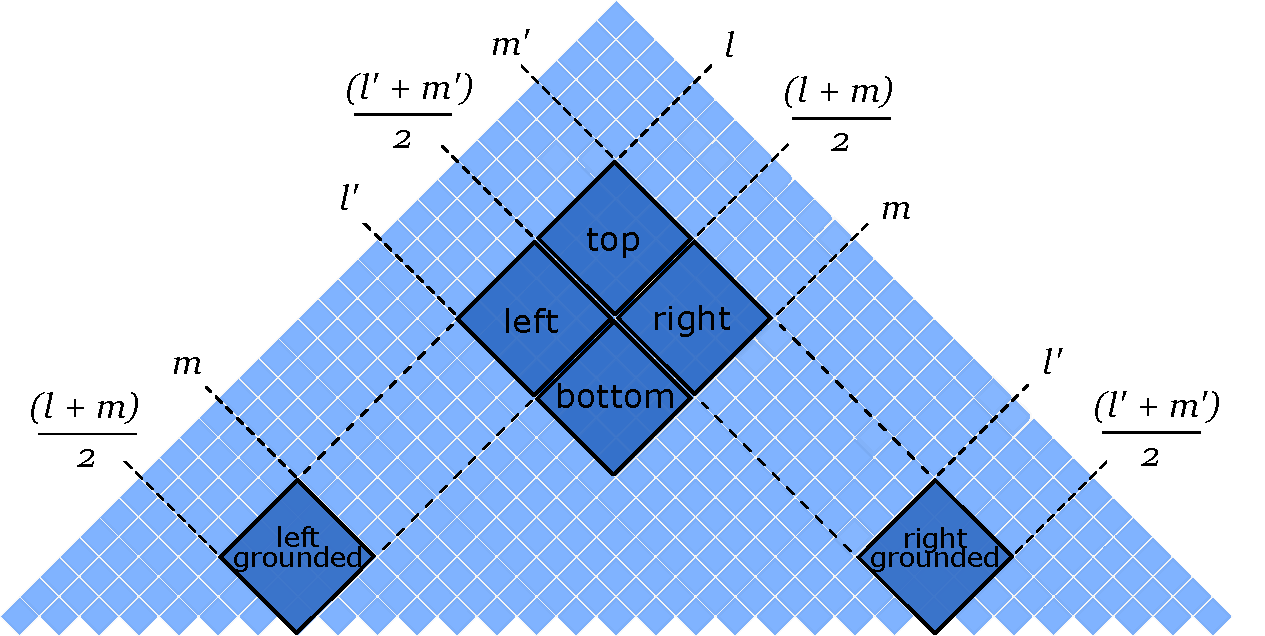
\includegraphics[width=6cm]{pictures/splitting_with_grounded.pdf}
        \caption{Matrix partition used in procedure \textit{complete(l, m, l', m')}}
        \label{fig1}
    \end{minipage}\hfill
    \begin{minipage}{0.48\textwidth}
        \centering
        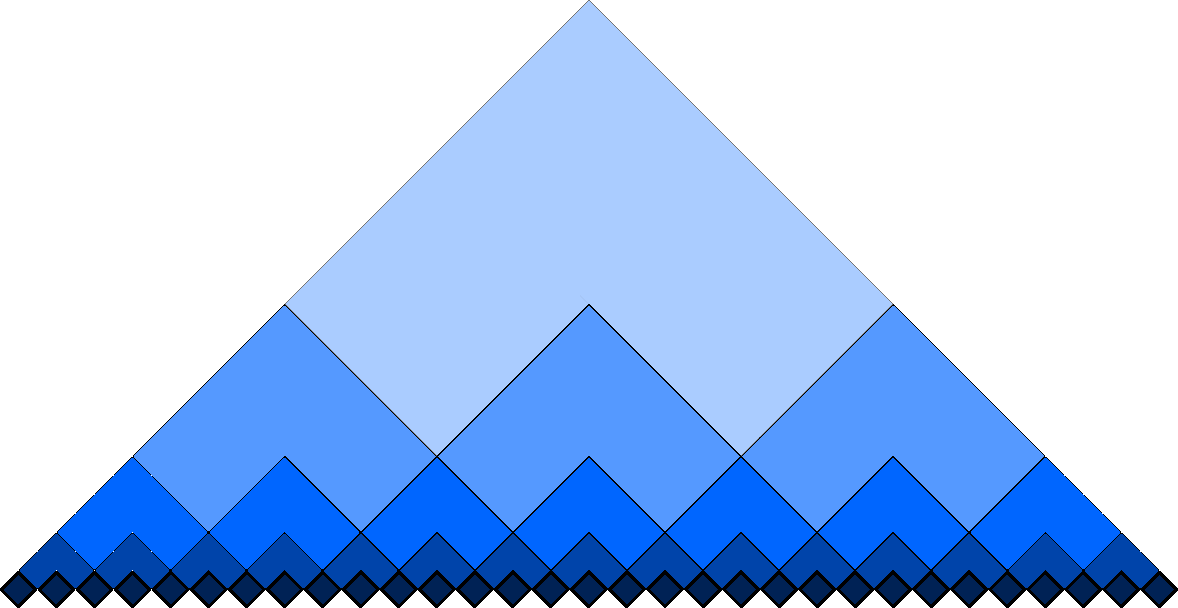
\includegraphics[width=6cm]{pictures/layers.pdf}
        \caption{Matrix partition on V-shaped layers used in modification}
        \label{fig2}
    \end{minipage}
 \end{center}
\vspace{-8mm}
\end{figure}

A simple example of parsing with the Valiant's algorithm is presented in Figure~\ref{fig3}.
Only several steps are shown, but it is enough to compare our version with the original algorithm.

\begin{figure}
\vspace{3mm}
 \begin{center}
 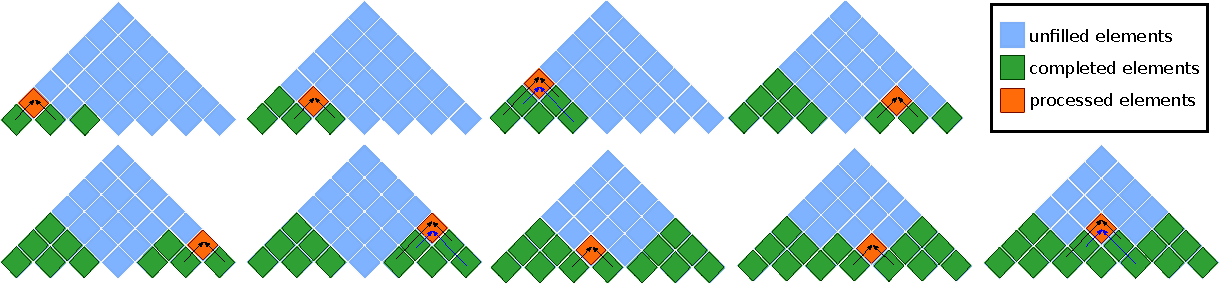
\includegraphics[width=12cm]{pictures/valbeg2.pdf}
    \caption{An example of beginning of Valiant's algorithm}
    \label{fig3}
\end{center}
\vspace{-8mm}
\end{figure}
\section{\bf Modified Valiant's algorithm}

In this section we describe the reorganization of submatrix processing order in the Valiant's algorithm which simplify independent handling of submatrices. As a result, proposed modification can facilitate implementation of parallel submatrix processing.

\subsection{\bf \it New approach}

The main change of this modification is the possibility to divide the parsing table into layers of disjoint submatrices of the same size.
The idea of division we have made from the reorganization of the matrix multiplication order is presented in figure~\ref{fig2}.
Each layer consists of square matrices which size is power of 2.
The layers are computed successively in the bottom-up order.
Each matrix in the layer can be handled independently, which can help to implement parallel version of layer processing function.

\begin{figure}[h]
\vspace{3mm}
 \begin{center}
 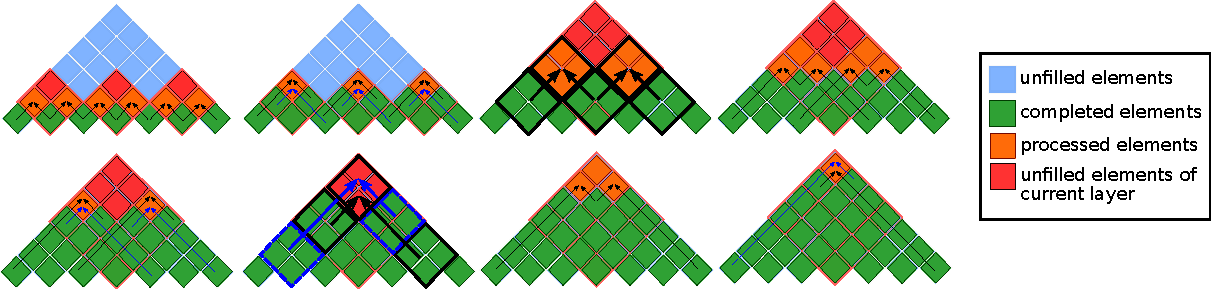
\includegraphics[width=12cm]{pictures/modivis2.pdf}
    \caption{An example of the modification of Valiant's algorithm}
    \label{fig4}
 \end{center}
\vspace{-8mm}
\end{figure}

A simple example of the modification is shown in figure~\ref{fig4}.
The lowest layer (submatrices which size is 1) is already computed and filling of the matrix starts with the second layer (subfigures 1-2).
Note that the same  process is presented in figure~\ref{fig3}, but here it can be done only in two steps using parallel computation of submatrix products.

The modified version of Valiant's algorithm is presented in listing~\ref{algo:modified}.
The procedure \textit{main()} computes the lowest layer $(T_{l, l+1})$, and then divide the table into layers, described earlier, and computes them through the \textit{completeVLayer()} call.
Thus, \textit{main()} computes all elements of parsing table $T$.
(Hereinafter, we use layer to mean set of submatrices.)

For brevity, we define \textit{left(subm), right(subm), top(subm), bottom(subm), \linebreak rightgrounded(subm)} and \textit{leftgrounded(subm)} functions which returns the submatrices for matrix $subm = (l, m, l', m')$ according to the original Valiant's algorithm (figure~\ref{fig2}).

Also denote some subsidiary functions for matrix layer $M$:
\begin{itemize}[noitemsep, nolistsep]
    \item[$-$] \textit{bottomsublayer(M)} $ = \{bottom(subm)\, |\,subm \in M \}$,
    \item[$-$] \textit{leftsublayer(M)} $ = \{\textit{left(subm)}\, |\,subm \in M \}$,
    \item[$-$] \textit{rightsublayer(M)} $ =\{\textit{right(subm)}\, |\,subm \in M \}$,
    \item[$-$] \textit{topsublayer(M)} $ = \{top(subm)\, |\,subm \in M \}$.
\end{itemize}

\begin{algorithm}[!h]
\SetAlgoNoLine
\KwIn{$G = (\Sigma, N, R, S), w = a_{1} \dots a_{n}, n \geq 1, n + 1 = 2^p, a_{i} \in \Sigma$ }
\underline{main()}{:}{

 \For {$l \in \{1, \ldots, n \}$}{$T_{l, l + 1} = \{A | A \rightarrow a_{l + 1} \in R\}$}
 \For{$1 \le i < p - 1 $}{
 layer = \textit{constructLayer(i)}\;
 \textit{completeVLayer(layer)}
 }
 accept if and only if $S \in T_{0, n}$
 \BlankLine
 }

\underline{constructLayer(i)}{:}{
 \BlankLine
 $\{(k2^i, (k+1)2^i, (k + 1)2^i, (k+2)2^i) \, |\, 0 \le k < 2^{p - i} - 1\}$
 \BlankLine
    }
\underline{completeLayer(M)}{:}{
\BlankLine
\If {$\forall (l, m, l', m') \in M \quad (m - l = 1)$}{\For{$ (l, m, l', m') \in M$}{$T_{l, l'} = f(P_{l, l'})$\;}}
\Else{
\textit{completeLayer(bottomsublayer(M))}\;
\textit{completeVLayer(M)}
}
\BlankLine
}

\underline{comleteVLayer(M)}{:}{
 \BlankLine
 \textit{multiplicationTasks$_1$ = \linebreak
    \{$left(subm)$, $leftgrounded(subm)$, $bottom(subm)\, |\,subm \in M \} \cup \linebreak  \{right(subm), bottom(subm), rightgrounded(subm)\, |\,subm \in M\}$\;}
 \BlankLine
 multiplicationTask$_2$ = $\{top(subm), leftgrounded(subm), right(subm)\, |\,subm \in M\}$\;
 \BlankLine
 multiplicationTask$_3$ = $\{top(subm), left(subm), rightgrounded\, |\,subm \in M\}$\;
 \BlankLine
 \textit{performMultiplications(multiplicationTask$_1$)}\;
 \textit{completeLayer(leftsublayer(M) $\cup$ rightsublayer(M))}\;
 \textit{performMultiplications(multiplicationTask$_2$)}\;
 \textit{performMultiplications(multiplicationTask$_3$)}\;
 \textit{completeLayer(topsublayer(M))}

 }
 \BlankLine

 \underline{performMultiplication(tasks)}{:}{\\
 \For{$ (m, m1, m2) \in \textit{tasks}$}{$P_{m} = P_{m} \cup (T_{m1} \times T_{m2})$\;}
 }

\caption{Parsing by matrix multiplication: Modified Version}
\label{algo:modified}
\end{algorithm}


The procedure \textit{completeVLayer(M)} takes an array of disjoint submatrices $M$ which represents a layer.
For each \textit{subm = (l, m, l', m') $\in M$} this procedure computes \textit{left(subm), right(subm), top(subm)}.
The procedure assumes that the elements of \textit{bottom(subm)} and $T_{i, j}$ for all $i$ and $j$ such that $l \leq i < j < m$ and $  l' \leq i < j < m'$ are already constructed.
Also it is assumed that the current value of
$P_{i, j} =  \{ (B, C) | \exists k, (m \le k < l'), a_{i + 1} \dots a_{k} \in L_G(B), a_{k + 1} \dots a_{j} \in L_G(C)\} $ for all $i$ and $j$ such that $l \leq i < m$ and $l' \leq j < m'$.

The procedure \textit{completeLayer(M)} also takes an array of disjoint submatrices $M$, but unlike the previous one, it computes $T_{i, j}$ for all $(i, j) \in subm$.
This procedure requires exactly same assumptions on $T_{i, j}$  and $P_{i, j}$  as in the previous case.

In the other words, \textit{completeVLayer(M)} computes the entire layer \textit{M} \linebreak and \textit{completeLayer($M_{2}$)} is a support function which is necessary for computation of smaller square submatrices $subm_{2} \in M_{2}$ inside of \textit{M}.

Finally, the procedure \textit{performMultiplication(tasks)}, where \textit{tasks} is an array of a triple of submatrices, perform basic step of algorithm: matrix multiplication. It is worth mentioning that, as distinct from the original algorithm, here $|tasks| \ge 1$ and each task can be computed independently.
So, practical implementation of this procedure can easily involve different techniques of parallel array processing, such as OpenMP~\ref{!!!}.

\subsection{\bf \it Algorithm for substrings}

Next we show how our modification can be applied to the string-matching problem.

So if we want to find all substrings of size $s$ which can be derived from a start symbol for an input string of size $n = 2^p$, we need to compute layers with submatrices of size not greater than $2^{l'}$, where $2^{l' - 2} < s \le 2^{l' - 1}$.

Let $l' = p - (m - 2)$ and consequently $(m - 2) = p - l'$.

For any  $m \le i \le p$ products of submatrices of size $2^{p - i}$ are calculated exactly $2^{2i - 1} - 2^{i}$ times and each of them imply multiplying $\mathcal{O}(|G|)$ Boolean submatrices.

\begin{equation}
\begin{array}{c}
C \sum\limits_{i=m}^p 2^{2i - 1} \cdot 2^{\omega(p - i)} \cdot f(2^{p - i}) =
C \cdot 2^{\omega l'}\sum\limits_{i=2}^{l'} 2^{(2 - \omega)i} \cdot 2^{2(p - l') - 1} \cdot f(2^{l' - i}) \le \\
C \cdot 2^{\omega l'} f(2^{l'}) \cdot 2^{2(p - l') - 1} \sum\limits_{i=2}^{l'} 2^{(2 - \omega)i} =
BMM(2^{l'}) \cdot 2^{2(p - l') - 1} \sum\limits_{i=2}^{l'} 2^{(2 - \omega)i}
\end{array}
\end{equation}

Thus, time complexity for searching all substrings is  $O(|G|BMM(2^{l'})(l' - 1))$, while time complexity for the full input string is $O(|G|BMM(2^p)(p - 1))$. In contract to the modification, Valiant's algorithm completely calculate at least 2 triangle submatrices of size $\frac{n}{2}$ (as shown in figure~\ref{fig5}) which mean minimum asymptotic complexity  $O(|G|BMM(2^{p - 1})(p - 2))$. Make a conclusion that the modification is asymptotically faster for substrings of size $s \ll n$  than the original algorithm.

\begin{figure}[h]
\vspace{3mm}
 \begin{center}
 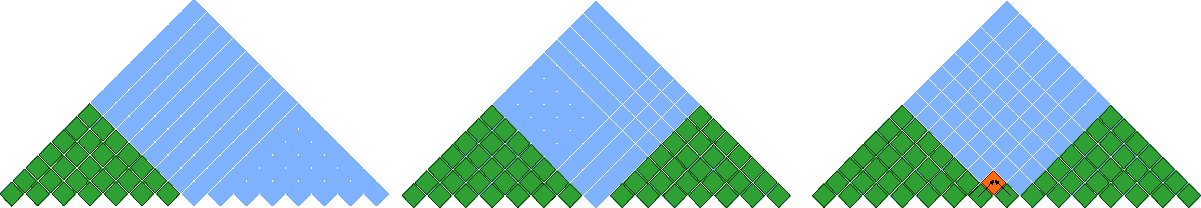
\includegraphics[width=12cm]{pictures/valsubstring.pdf}
    \caption{The number of elements necessary to compute in Valiant's algorithm. That means it is nessesary to calculate at least 2 triangle submatrices of size $\frac{n}{2}$.}
    \label{fig5}
 \end{center}
\vspace{-8mm}
\end{figure}

\section{Conclusion and future work}
In this paper, we shown how the context-free path query evaluation w.r.t. the relational and the single-path query semantics can be reduced to the calculation of matrix transitive closure. Also, we provided a formal proof of the correctness of the proposed reduction. In addition, we introduced an algorithm for computing this transitive closure, which allows us to efficiently apply GPGPU computing techniques. Finally, we shown the practical applicability of the proposed algorithm by running different implementations of our algorithm on real-world data.

We can identify several open problems for further research. In this paper we have considered only two semantics of context-free path querying but there are other important semantics, such as all-path query semantics~\cite{hellingsPathQuerying} which requires to present all paths for all triples $(A,m,n)$. Context-free path querying implemented with algorithm~\cite{GLL} can answer the queries in all-path query semantics by constructing a parse forest. It is possible to construct a parse forest for a linear input by matrix multiplication~\cite{okhotin_cyk}. Whether it is possible to generalize this approach for a graph input is an open question.

In our algorithm, we calculate the matrix transitive closure naively, but there are algorithms for the transitive closure calculation, which are asymptotically more efficient. Therefore, the question is whether it is possible to apply these algorithms for the matrix transitive closure calculation to the problem of context-free path querying.

Also, there are Boolean grammars~\cite{okhotinBoolean}, which have more expressive power than context-free grammars. Boolean path querying is an undecidable problem~\cite{hellingsRelational} but our algorithm can be trivially generalized to work on boolean grammars because parsing with boolean grammars can be expressed by matrix multiplication~\cite{okhotin_cyk}. It is not clear what a result of our algorithm applied to Boolean grammars would look like. Our hypothesis is that it would produce the upper approximation of a solution.

From a practical point of view, matrix multiplication in the main loop of the proposed algorithm may be performed on different GPGPU independently. It can help to utilize the power of multi-GPU systems and increase the performance of context-free path querying.

There is an algorithm~\cite{apspGPU} for transitive closure calculation on directed graphs which generalized to handle graph sizes inherently larger then the DRAM memory available on the GPU. Therefore, the question is whether it is possible to apply this approach to the matrix transitive closure calculation in the problem of context-free path querying.


\section*{\bf Acknowledgments}

The research was supported by the Russian Science Foundation grant 18-11-00100 and a grant from JetBrains Research.


%\bibliographystyle{apalike}
\bibliographystyle{ieeetr}

{\fontsize{10}{10}\selectfont
%\begin{thebibliography}{99}
\setlength{\parskip}{0pt}

\bibliography{main}

%\end{thebibliography}
}

\end{document}
